\documentclass[12pt,a4paper]{article}

% ─── Page Layout ───────────────────────────────────────────────────────────────
\usepackage[a4paper, margin=0.8in, headheight=14pt]{geometry}

% ─── Fonts (XeLaTeX) ───────────────────────────────────────────────────────────
\usepackage{fontspec}
\usepackage{unicode-math}
\setmainfont{TeX Gyre Pagella}
\setmonofont[Scale=0.88]{TeX Gyre Cursor}
\setmathfont{Latin Modern Math}

% ─── Packages ──────────────────────────────────────────────────────────────────
\usepackage{xcolor}
\usepackage{colortbl}
\usepackage{titlesec}
\usepackage{enumitem}
\usepackage{tabularx}
\usepackage{booktabs}
\usepackage{array}
\usepackage{amsmath}
\usepackage{tikz}
\usetikzlibrary{shapes.geometric, arrows.meta, positioning, calc, fit, decorations.pathreplacing}
\usepackage{tcolorbox}
\tcbuselibrary{skins, breakable}
\usepackage{hyperref}
\usepackage{fancyhdr}
\usepackage{graphicx}
\usepackage{microtype}
\hyphenpenalty=10000
\exhyphenpenalty=10000
\sloppy
\usepackage{caption}
\usepackage{setspace}
\usepackage{multirow}
\usepackage{tocloft}

% ─── Q&A helper ────────────────────────────────────────────────────────────────
\newcommand{\Q}[1]{\textbf{#1}\par\noindent\ignorespaces}

% ─── Colour Palette ────────────────────────────────────────────────────────────
\definecolor{myred}{RGB}{196,30,58}
\definecolor{mydark}{RGB}{30,30,50}
\definecolor{mygreen}{RGB}{14,120,80}
\definecolor{myteal}{RGB}{0,130,140}
\definecolor{myamber}{RGB}{180,100,0}
\definecolor{mypurple}{RGB}{100,30,160}
\definecolor{mygray}{RGB}{246,247,249}
\definecolor{mgframe}{RGB}{180,185,200}
\definecolor{watermark}{RGB}{145,150,170}
\definecolor{hdrred}{RGB}{250,232,235}
\definecolor{hdrgreen}{RGB}{220,244,233}
\definecolor{hdrteal}{RGB}{220,242,244}
\definecolor{hdramber}{RGB}{253,242,215}
\definecolor{hdrpurple}{RGB}{238,228,255}
\definecolor{hdrgray}{RGB}{238,240,245}
\definecolor{rowalt}{RGB}{250,251,253}

% ─── Section Formatting ────────────────────────────────────────────────────────
\titleformat{\section}
  {\large\bfseries\color{myred}}{\thesection.}{0.5em}{}
  [\vspace{1pt}{\color{myred}\rule{\linewidth}{0.8pt}}]
\titleformat{\subsection}
  {\normalsize\bfseries\color{myteal}}{\thesubsection}{0.5em}{}
\titlespacing*{\section}{0pt}{18pt}{7pt}
\titlespacing*{\subsection}{0pt}{11pt}{4pt}

% ─── Paragraph ─────────────────────────────────────────────────────────────────
\setlength{\parindent}{0pt}
\setlength{\parskip}{4pt}

% ─── TOC Styling ───────────────────────────────────────────────────────────────
\renewcommand{\cfttoctitlefont}{\large\bfseries\color{myred}}
\renewcommand{\cftaftertoctitle}{\par\noindent{\color{myred}\rule{\linewidth}{0.8pt}}}
\setlength{\cftbeforetoctitleskip}{0pt}
\setlength{\cftaftertoctitleskip}{6pt}
\renewcommand{\cftsecfont}{\normalsize\bfseries\color{mydark}}
\renewcommand{\cftsecpagefont}{\normalsize\bfseries\color{mydark}}
\renewcommand{\cftsecleader}{\cftdotfill{\cftdotsep}}
\setlength{\cftbeforesecskip}{7pt}
\renewcommand{\cftsubsecfont}{\small\color{mydark}}
\renewcommand{\cftsubsecpagefont}{\small\color{mydark}}
\setlength{\cftbeforesubsecskip}{3pt}
\setlength{\cftsubsecindent}{1.4em}

% ─── Table helpers ─────────────────────────────────────────────────────────────
\renewcommand{\arraystretch}{1.45}
\setlength{\tabcolsep}{6pt}
\arrayrulecolor{mydark}
\newcolumntype{B}[1]{>{\small\bfseries\raggedright\arraybackslash}m{#1}}
\newcolumntype{Y}{>{\small\raggedright\arraybackslash}X}
\renewcommand{\tabularxcolumn}[1]{m{#1}}

% ─── Header / Footer ───────────────────────────────────────────────────────────
\pagestyle{fancy}
\fancyhf{}
\fancyhead[L]{\small\color{myred}\textbf{PE-EC702B}\;\color{mydark}--- Digital Image and Video Processing}
\fancyhead[R]{\small\color{myteal}\textbf{Module 4 Notes}}
\fancyfoot[C]{\small\color{mydark}\thepage}
\fancyfoot[R]{\small\color{watermark}\textit{\copyright\ Biraj}}
\renewcommand{\headrulewidth}{0.5pt}
\renewcommand{\footrulewidth}{0.3pt}

% ─── Hyperref ──────────────────────────────────────────────────────────────────
\hypersetup{
  colorlinks=true, linkcolor=myteal, urlcolor=myteal,
  pdfauthor={Biraj Sarkar},
  pdftitle={PE-EC702B --- Module 4 Notes}
}

% ─── tcolorbox styles ──────────────────────────────────────────────────────────
\tcbset{
  tikzbox/.style={
    colback=mygray, colframe=mgframe, boxrule=0.6pt, arc=4pt,
    left=8pt, right=8pt, top=6pt, bottom=6pt,
    colbacktitle=mgframe, coltitle=mydark,
    fonttitle=\small\bfseries
  },
  defbox/.style={
    colback=hdrgreen, colframe=mygreen, boxrule=0.8pt, arc=4pt,
    left=9pt, right=9pt, top=6pt, bottom=6pt,
    colbacktitle=mygreen, coltitle=white,
    fonttitle=\small\bfseries
  },
  formulabox/.style={
    colback=hdrteal, colframe=myteal, boxrule=0.8pt, arc=4pt,
    left=9pt, right=9pt, top=7pt, bottom=7pt,
    colbacktitle=myteal, coltitle=white,
    fonttitle=\small\bfseries
  },
  examplebox/.style={
    colback=hdramber, colframe=myamber, boxrule=0.8pt, arc=4pt,
    left=9pt, right=9pt, top=6pt, bottom=6pt,
    colbacktitle=myamber, coltitle=white,
    fonttitle=\small\bfseries,
    breakable
  },
  masonbox/.style={
    colback=hdrpurple, colframe=mypurple, boxrule=0.8pt, arc=4pt,
    left=9pt, right=9pt, top=6pt, bottom=6pt,
    colbacktitle=mypurple, coltitle=white,
    fonttitle=\small\bfseries
  },
  exambox/.style={
    colback=hdrpurple, colframe=mypurple, boxrule=1pt, arc=5pt,
    left=10pt, right=10pt, top=8pt, bottom=8pt,
    colbacktitle=mypurple, coltitle=white,
    fonttitle=\bfseries,
    breakable, title after break={\textbf{Frequently Asked / Viva Questions (contd.)}}}
}
\tcbset{breakable}

% ─── TikZ styles ───────────────────────────────────────────────────────────────
\tikzset{
  block/.style={rectangle, draw=myteal, fill=hdrteal,
    text width=2.1cm, align=center, minimum height=0.85cm,
    font=\small, rounded corners=3pt, line width=0.7pt},
  arrow/.style={-Stealth, thick, color=mydark},
  line/.style={thick, color=mydark}
}

% ═══════════════════════════════════════════════════════════════════════════════
\begin{document}
% ═══════════════════════════════════════════════════════════════════════════════

\begin{center}
  {\LARGE\bfseries\color{myred} PE-EC702B --- Digital Image and Video Processing}\\[5pt]
  {\normalsize\color{mydark} Semester VII \quad$\bullet$\quad 3L:0T:0P \quad$\bullet$\quad 3 Credits}\\[3pt]
  {\normalsize\color{myteal}\textbf{Module 4 Exam Notes: Image Segmentation}}\\[3pt]
  {\small\color{mydark} CGEC \;$|$\; B.Tech ECE (2023--27) \;$|$\; \textit{Biraj Sarkar}}
\end{center}
\vspace{2pt}
\noindent{\color{myred}\rule{\linewidth}{1.5pt}}
\vspace{2pt}

\hypersetup{linkcolor=mydark}
\tableofcontents
\hypersetup{linkcolor=myteal}
\newpage

% ===============================================================================
\section{Detection of Discontinuities}
% ===============================================================================

Image segmentation is based on one of two basic properties of intensity values: discontinuity (partitioning based on abrupt changes) or similarity (partitioning into homogeneous regions).

\begin{tcolorbox}[defbox, title={Edge and Line Detection}]
\textbf{Edge Detection:} The process of locating boundaries where intensity changes rapidly. These are classified as step edges (ideal abrupt transitions) or ramp edges (gradual, practical transitions due to blur).
\end{tcolorbox}

\subsection{Canny Edge Detection Algorithm}
The Canny detector is considered the optimal edge detector due to its low error rate, precise edge localization, and single response constraint.
\begin{enumerate}[leftmargin=*, itemsep=3.5pt]
  \item \textbf{Noise Reduction:} Smooth the image with a 2D Gaussian filter to eliminate high-frequency noise.
  \item \textbf{Gradient Computation:} Compute the local gradient magnitude $M(x,y)$ and direction $\alpha(x,y)$ using Sobel or Prewitt masks.
  \item \textbf{Non-Maximum Suppression (NMS):} Thin the thick edges by checking if the gradient magnitude at a pixel is a local maximum in the direction of the gradient. If not, set it to zero.
  \item \textbf{Hysteresis Thresholding:} Use two thresholds, $T_{\text{high}}$ and $T_{\text{low}}$:
    \begin{itemize}[leftmargin=1em, itemsep=1pt]
      \item Pixels $> T_{\text{high}}$ are marked as strong edges (always kept).
      \item Pixels $< T_{\text{low}}$ are suppressed.
      \item Pixels in-between are marked as weak edges and kept only if they are connected to a strong edge.
    \end{itemize}
\end{enumerate}

% ===============================================================================
\section{Edge Linking and Boundary Detection}
% ===============================================================================

Since noise and lighting can cause breaks in detected edges, edge linking is used to group pixels into meaningful boundaries.

\subsection{Hough Transform}
The Hough Transform groups edge pixels by determining if they lie on a curve of specified shape (typically a straight line).

\begin{tcolorbox}[formulabox, title={Hough Transform Formulations}]
A straight line in Cartesian coordinates is $y = mx + c$.
\par\noindent
In Hough parameter space, every point $(x,y)$ maps to a line in $(m,c)$ space:
\begin{equation}
  c = -x m + y
\end{equation}
However, vertical lines have infinite slope ($m \to \infty$). To resolve this, we use the polar representation:
\begin{equation}
  \rho = x \cos\theta + y \sin\theta
\end{equation}
where $\rho$ is the perpendicular distance from the origin to the line, and $\theta$ is the angle of the normal vector relative to the $x$-axis.
\par\noindent
\textbf{Algorithm:}
\begin{enumerate}[leftmargin=*, itemsep=2pt]
  \item Quantize the parameter space $(\rho, \theta)$ into an accumulator grid.
  \item For each edge pixel $(x_i, y_i)$ in the image, vary $\theta$ over the range $[-90^\circ, 90^\circ]$ and compute the corresponding $\rho$.
  \item Increment the accumulator cell: $A(\rho, \theta) = A(\rho, \theta) + 1$.
  \item Local maxima (peaks) in the accumulator grid indicate lines in the image.
\end{enumerate}
\end{tcolorbox}

% ===============================================================================
\section{Thresholding}
% ===============================================================================

Thresholding converts a grayscale image $f(x,y)$ into a binary image $g(x,y)$ based on intensity.

\subsection{Global vs. Local Adaptive Thresholding}
\begin{itemize}[leftmargin=*, itemsep=3.5pt]
  \item \textbf{Global Thresholding:} A single threshold $T$ is used for the entire image:
    \begin{equation}
      g(x,y) = \begin{cases} 1 & \text{if } f(x,y) > T \\ 0 & \text{if } f(x,y) \le T \end{cases}
    \end{equation}
    Only effective if the image has a bimodal histogram and uniform illumination.
  \item \textbf{Local/Adaptive Thresholding:} The threshold $T(x,y)$ changes dynamically across the image based on local neighborhood statistics (e.g., local mean or local standard deviation), resolving non-uniform illumination.
\end{itemize}

\subsection{Otsu's Optimum Thresholding Method}
Otsu's method automatically selects the optimal global threshold $T$ by maximizing the \textbf{between-class variance} $\sigma_B^2$ of the two pixel classes (background $C_1$ and foreground $C_2$).

\begin{tcolorbox}[formulabox, title={Otsu's Formulation}]
Let $P_1(T)$ and $P_2(T)$ be the probabilities of the two classes separated by threshold $T$, and let $\mu_1(T)$ and $\mu_2(T)$ be their mean intensities.
\par\noindent
The between-class variance $\sigma_B^2(T)$ is defined as:
\begin{equation}
  \sigma_B^2(T) = P_1(T) P_2(T) \left[ \mu_1(T) - \mu_2(T) \right]^2
\end{equation}
We evaluate $\sigma_B^2(T)$ for all possible gray levels $T \in [0, L-1]$. The optimum threshold $T^*$ is the value that maximizes this variance:
\begin{equation}
  T^* = \arg\max_{0 \le T \le L-1} \sigma_B^2(T)
\end{equation}
\end{tcolorbox}

% ===============================================================================
\section{Region-Based Segmentation}
% ===============================================================================

Region-based segmentation groups pixels directly into regions based on similarity.

\begin{itemize}[leftmargin=*, itemsep=3.5pt]
  \item \textbf{Region Growing:} Starts with seed points and appends adjacent pixels to the region if they satisfy homogeneity criteria (e.g., color, texture, intensity).
  \item \textbf{Region Splitting and Merging:}
    \begin{itemize}[leftmargin=1em, itemsep=1.5pt]
      \item Start with the entire image region $R$.
      \item If $R$ does not satisfy the homogeneity criterion $P(R) = \text{True}$ (e.g., variance too high), split it into four disjoint quadrants.
      \item Recursively split non-homogeneous quadrants. This is modeled by a \textbf{quadtree} hierarchy.
      \item After splitting ceases, merge adjacent quadrants $R_i$ and $R_j$ if their union satisfies the homogeneity criterion ($P(R_i \cup R_j) = \text{True}$).
    \end{itemize}
\end{itemize}

\begin{tcolorbox}[tikzbox, title={Quadtree Decomposition for Splitting and Merging}]
\centering
\begin{minipage}{0.42\textwidth}
  \centering
  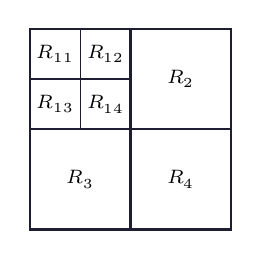
\begin{tikzpicture}[scale=0.85, every node/.style={font=\scriptsize}]
    % Partitioned Image
    \draw[thick, color=mydark] (0,0) rectangle (3,3);
    \draw[thick, color=mydark] (1.5,0) -- (1.5,3);
    \draw[thick, color=mydark] (0,1.5) -- (3,1.5);
    
    % Split top-left block (R1) into 4
    \draw[thin, color=mydark] (0.75, 1.5) -- (0.75, 3.0);
    \draw[thin, color=mydark] (0, 2.25) -- (1.5, 2.25);
    
    % Labels
    \node at (0.375, 2.625) {$R_{11}$};
    \node at (1.125, 2.625) {$R_{12}$};
    \node at (0.375, 1.875) {$R_{13}$};
    \node at (1.125, 1.875) {$R_{14}$};
    \node at (2.25, 2.25) {$R_2$};
    \node at (0.75, 0.75) {$R_3$};
    \node at (2.25, 0.75) {$R_4$};
  \end{tikzpicture}
  \par\vspace{2pt}\small\textbf{Image Partitions}
\end{minipage}
\hfill
\begin{minipage}{0.54\textwidth}
  \centering
  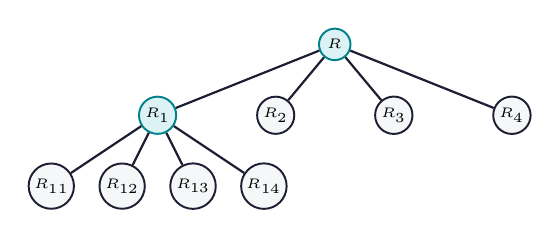
\begin{tikzpicture}[scale=1.0, every node/.style={font=\scriptsize}]
    \tikzset{
      tnode/.style={circle, draw=myteal, fill=hdrteal, minimum size=0.4cm, inner sep=1.2pt, font=\tiny\bfseries, line width=0.7pt},
      leaf/.style={circle, draw=mydark, fill=mygray, minimum size=0.4cm, inner sep=1.2pt, font=\tiny, line width=0.7pt}
    }
    
    % Root Node
    \node[tnode] (root) at (0,0) {$R$};
    
    % Level 1
    \node[tnode] (r1) at (-2.25, -0.9) {$R_1$};
    \node[leaf]  (r2) at (-0.75, -0.9) {$R_2$};
    \node[leaf]  (r3) at (0.75, -0.9) {$R_3$};
    \node[leaf]  (r4) at (2.25, -0.9) {$R_4$};
    
    \draw[line] (root) -- (r1);
    \draw[line] (root) -- (r2);
    \draw[line] (root) -- (r3);
    \draw[line] (root) -- (r4);
    
    % Level 2 (under R1)
    \node[leaf] (r11) at (-3.6, -1.8) {$R_{11}$};
    \node[leaf] (r12) at (-2.7, -1.8) {$R_{12}$};
    \node[leaf] (r13) at (-1.8, -1.8) {$R_{13}$};
    \node[leaf] (r14) at (-0.9, -1.8) {$R_{14}$};
    
    \draw[line] (r1) -- (r11);
    \draw[line] (r1) -- (r12);
    \draw[line] (r1) -- (r13);
    \draw[line] (r1) -- (r14);
  \end{tikzpicture}
  \par\vspace{2pt}\small\textbf{Quadtree Hierarchy}
\end{minipage}
\end{tcolorbox}

% ===============================================================================
\section{Worked Examples}
% ===============================================================================

\begin{tcolorbox}[examplebox, title={Hough Transform Line Mapping}]
\textbf{Problem:} Map the edge point $p(1,1)$ in Cartesian coordinates into Hough parameter space $(\rho, \theta)$. Specifically, calculate the values of $\rho$ for $\theta = -45^\circ$, $0^\circ$, $45^\circ$, and $90^\circ$.

\par\noindent\rule{\linewidth}{0.5pt}\par
\textbf{Solution:}
We use the polar line equation: $\rho = x \cos\theta + y \sin\theta$.
Given $x = 1$ and $y = 1$:
\begin{equation*}
  \rho(\theta) = 1 \cdot \cos\theta + 1 \cdot \sin\theta = \cos\theta + \sin\theta
\end{equation*}

Let's compute the value of $\rho$ for each requested angle $\theta$:
\begin{enumerate}[leftmargin=*, itemsep=3.5pt]
  \item \textbf{For $\theta = -45^\circ$:}
    \begin{align*}
      \cos(-45^\circ) &= \cos(45^\circ) = \frac{1}{\sqrt{2}} \approx 0.707 \\
      \sin(-45^\circ) &= -\sin(45^\circ) = -\frac{1}{\sqrt{2}} \approx -0.707 \\
      \rho &= 0.707 - 0.707 = 0
    \end{align*}
  \item \textbf{For $\theta = 0^\circ$:}
    \begin{align*}
      \cos(0^\circ) &= 1, \quad \sin(0^\circ) = 0 \\
      \rho &= 1 + 0 = 1
    \end{align*}
  \item \textbf{For $\theta = 45^\circ$:}
    \begin{align*}
      \cos(45^\circ) &= \frac{1}{\sqrt{2}} \approx 0.707, \quad \sin(45^\circ) = \frac{1}{\sqrt{2}} \approx 0.707 \\
      \rho &= 0.707 + 0.707 = 1.414 = \sqrt{2}
    \end{align*}
  \item \textbf{For $\theta = 90^\circ$:}
    \begin{align*}
      \cos(90^\circ) &= 0, \quad \sin(90^\circ) = 1 \\
      \rho &= 0 + 1 = 1
    \end{align*}
\end{enumerate}

\par\noindent\textbf{Resulting Hough Curves points:}
The Cartesian point $(1,1)$ maps to the sinusoidal curve in $(\rho, \theta)$ space passing through the coordinates:
\begin{equation*}
  (-45^\circ, 0), \quad (0^\circ, 1), \quad (45^\circ, \sqrt{2}), \quad (90^\circ, 1)
\end{equation*}
\end{tcolorbox}

\newpage

% ===============================================================================
% MANDATORY QUICK REVISION PAGE
% ===============================================================================
\begin{center}
  {\large\bfseries\color{myred} Quick Revision --- Module IV}\\[3pt]
  {\small\color{mydark} Image Segmentation $|$ PE-EC702B}
\end{center}
\noindent{\color{myred}\rule{\linewidth}{1.2pt}}
\vspace{4pt}

\begin{tcolorbox}[formulabox, title={\textbf{Key Formulas at a Glance}}]
\renewcommand{\arraystretch}{1.3}
\begin{tabularx}{\linewidth}{B{5.0cm} X}
Polar Line Equation & $\rho = x \cos\theta + y \sin\theta$ \\
Global Thresholding & $g(x,y) = \begin{cases} 1 & \text{if } f(x,y) > T \\ 0 & \text{if } f(x,y) \le T \end{cases}$ \\
Otsu's Class Probabilities & $P_1(T) = \sum_{i=0}^T p_i, \quad P_2(T) = 1 - P_1(T)$ \\
Otsu's Between-Class Var & $\sigma_B^2(T) = P_1(T) P_2(T) [\mu_1(T) - \mu_2(T)]^2$ \\
Canny Gaussian Smoothing & $G(x,y) = \frac{1}{2\pi \sigma^2} e^{-(x^2+y^2)/2\sigma^2}$ \\
Sobel Gradient Magnitude & $M(x,y) = \sqrt{G_x^2 + G_y^2} \approx |G_x| + |G_y|$
\end{tabularx}
\tcbset{colbacktitle=myteal, coltitle=white}
\end{tcolorbox}

\begin{tcolorbox}[defbox, title={\textbf{One-Line Definitions}}]
\begin{itemize}[leftmargin=*, itemsep=2.5pt, topsep=0pt]
  \item \textbf{Hysteresis Thresholding:} A dual-threshold edge linking method that retains weak edges only if connected to strong ones.
  \item \textbf{Hough Transform:} A global parameter mapping technique used to detect straight lines or shapes from broken edge segments.
  \item \textbf{Adaptive Thresholding:} Thresholding where $T$ varies across the image to accommodate local illumination changes.
  \item \textbf{Otsu's Method:} An optimal global thresholding algorithm that automatically chooses $T$ to maximize between-class variance.
  \item \textbf{Quadtree:} A tree data structure in which each internal node has exactly four children, used for image partitioning.
  \item \textbf{Non-Maximum Suppression:} An edge-thinning technique that suppresses non-peak gradient magnitudes along gradient directions.
\end{itemize}
\end{tcolorbox}

\begin{tcolorbox}[exambox, title={\textbf{Frequently Asked / Viva Questions}}]
\begin{enumerate}[leftmargin=*, itemsep=3.5pt, label=\arabic*.]
  \item \Q{State the three optimal criteria defined by Canny for edge detection.} (1) Low error rate (no missed or false edges), (2) Good localization (minimum distance between real and detected edges), and (3) Single response (only one detector response per edge).
  \item \Q{Why is polar representation ($\rho, \theta$) preferred over slope-intercept ($m,c$) in the Hough Transform?} The slope $m$ approaches infinity for vertical lines, requiring infinite storage size. Polar parameters are bounded: $\theta \in [-90^\circ, 90^\circ]$ and $\rho \in [-D, D]$ (where $D$ is the image diagonal).
  \item \Q{How does Otsu's algorithm select the threshold value?} It computes the between-class variance $\sigma_B^2(T)$ for every possible threshold value $T \in [0, L-1]$, and selects $T^*$ that yields the maximum between-class variance.
  \item \Q{What is the physical meaning of maximizing between-class variance in thresholding?} Maximizing between-class variance minimizes the spread (within-class variance) of background and foreground pixels, maximizing their statistical separation.
  \item \Q{Explain the region splitting and merging algorithm.} The entire image is recursively split into quadrants if it fails a homogeneity test (variance too high). After splitting ceases, adjacent quadrants that satisfy the homogeneity test are merged.
  \item \Q{What is the effect of noise on global thresholding?} Noise distorts the bimodal histogram valleys, causing global thresholding to create false boundaries and merge background and foreground details.
  \item \Q{What is the function of the Gaussian filter in Canny edge detection?} The Gaussian filter acts as a low-pass filter, smoothing out high-frequency noise which would otherwise cause false edge detections during derivative operations.
  \item \Q{What are weak edges in Canny edge detection?} Weak edges are edge candidates with gradient magnitudes between $T_{\text{low}}$ and $T_{\text{high}}$. They are kept only if they connect to a strong edge.
  \item \Q{Define region growing.} It is a segmentation procedure that groups pixels into larger regions starting from predefined seed points by adding neighboring pixels that satisfy similarity criteria.
  \item \Q{How does Sobel gradient calculation differ from Laplacian edge detection?} Sobel uses first derivatives (showing direction and magnitude, robust to noise), while Laplacian uses second derivatives (isotropic, thinned edges, but highly sensitive to noise).
\end{enumerate}
\tcbset{colbacktitle=myteal, coltitle=white}
\end{tcolorbox}

\begin{tcolorbox}[tikzbox, title={Edge-Based vs. Region-Based Segmentation}]
\centering
\renewcommand{\arraystretch}{1.2}
\begin{tabularx}{\linewidth}{>{\bfseries}B{3.2cm} Y Y}
Attribute & Edge-Based Segmentation & Region-Based Segmentation \\
\midrule
Primary Property & Discontinuity of intensity features & Similarity / Homogeneity of regions \\
Noise Sensitivity & High (sensitive to noise and gaps) & Low (integrates spatial neighborhood) \\
Open Boundaries & Yes (requires edge linking) & No (always yields closed regions) \\
\bottomrule
\end{tabularx}
\tcbset{colbacktitle=myteal, coltitle=white}
\end{tcolorbox}

\end{document}
